\documentclass{standalone}
\usepackage{tikz}
\usetikzlibrary{patterns, positioning}

\begin{document}
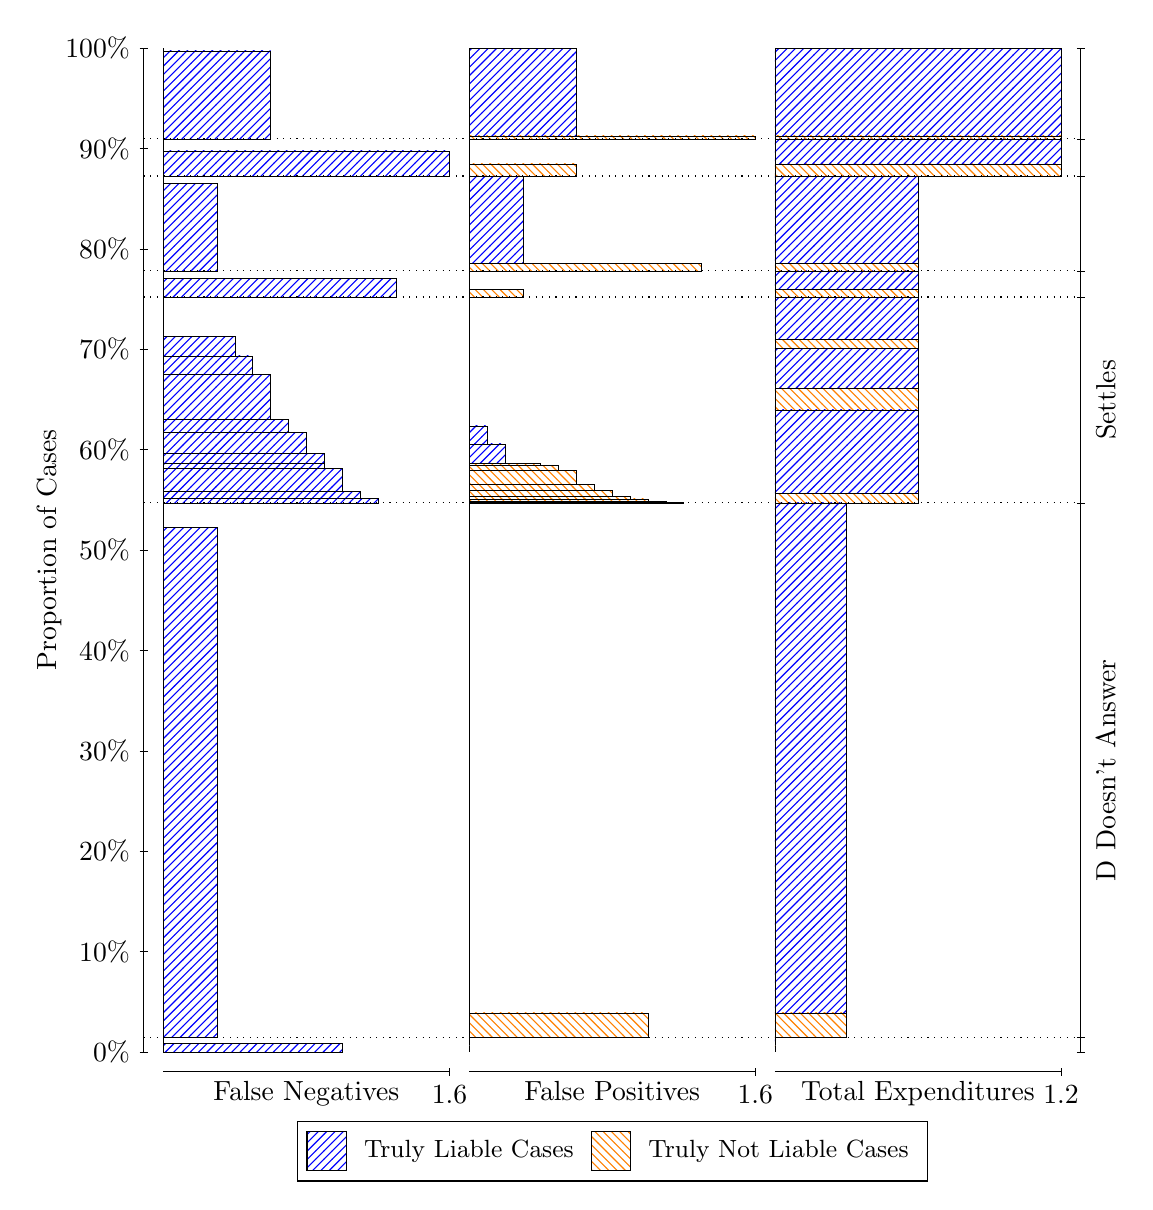
\begin{tikzpicture}
\draw[black, very thin] (1.5,1.75) -- (1.5,14.5);
\node[rotate=90, anchor=center] at (0.3, 8.125) {Proportion of Cases};
\draw[black, very thin] (1.45,1.75) -- (1.55,1.75);
\node[anchor=east] at (1.45, 1.75) {0\%};
\draw[black, very thin] (1.45,3.025) -- (1.55,3.025);
\node[anchor=east] at (1.45, 3.025) {10\%};
\draw[black, very thin] (1.45,4.3) -- (1.55,4.3);
\node[anchor=east] at (1.45, 4.3) {20\%};
\draw[black, very thin] (1.45,5.575) -- (1.55,5.575);
\node[anchor=east] at (1.45, 5.575) {30\%};
\draw[black, very thin] (1.45,6.85) -- (1.55,6.85);
\node[anchor=east] at (1.45, 6.85) {40\%};
\draw[black, very thin] (1.45,8.125) -- (1.55,8.125);
\node[anchor=east] at (1.45, 8.125) {50\%};
\draw[black, very thin] (1.45,9.4) -- (1.55,9.4);
\node[anchor=east] at (1.45, 9.4) {60\%};
\draw[black, very thin] (1.45,10.675) -- (1.55,10.675);
\node[anchor=east] at (1.45, 10.675) {70\%};
\draw[black, very thin] (1.45,11.95) -- (1.55,11.95);
\node[anchor=east] at (1.45, 11.95) {80\%};
\draw[black, very thin] (1.45,13.225) -- (1.55,13.225);
\node[anchor=east] at (1.45, 13.225) {90\%};
\draw[black, very thin] (1.45,14.5) -- (1.55,14.5);
\node[anchor=east] at (1.45, 14.5) {100\%};

\draw[black, very thin] (13.4,1.75) -- (13.4,14.5);
\draw[black, very thin] (13.35,1.75) -- (13.45,1.75);
\node[anchor=west] at (13.35, 1.75) {};
\draw[black, very thin] (13.35,1.9347) -- (13.45,1.9347);
\node[anchor=west] at (13.35, 1.9347) {};
\draw[black, very thin] (13.35,8.7245) -- (13.45,8.7245);
\node[anchor=west] at (13.35, 8.7245) {};
\draw[black, very thin] (13.35,11.338) -- (13.45,11.338);
\node[anchor=west] at (13.35, 11.338) {};
\draw[black, very thin] (13.35,11.671) -- (13.45,11.671);
\node[anchor=west] at (13.35, 11.671) {};
\draw[black, very thin] (13.35,12.875) -- (13.45,12.875);
\node[anchor=west] at (13.35, 12.875) {};
\draw[black, very thin] (13.35,13.347) -- (13.45,13.347);
\node[anchor=west] at (13.35, 13.347) {};
\draw[black, very thin] (13.35,14.5) -- (13.45,14.5);
\node[anchor=west] at (13.35, 14.5) {};

\draw[black, very thin, pattern color=blue, pattern=north east lines] (1.75,1.75) rectangle (4.0208,1.8544);
\draw[black, very thin, pattern color=orange, pattern=north west lines] (1.75,1.8544) rectangle (1.75,1.9347);
\draw[black, very thin, pattern color=blue, pattern=north east lines] (1.75,1.9347) rectangle (2.4312,8.4139);
\draw[black, very thin, pattern color=orange, pattern=north west lines] (1.75,8.4139) rectangle (1.75,8.7245);
\draw[black, very thin, pattern color=blue, pattern=north east lines] (1.75,8.7245) rectangle (4.475,8.7773);
\draw[black, very thin, pattern color=blue, pattern=north east lines] (1.75,8.7773) rectangle (4.2479,8.874);
\draw[black, very thin, pattern color=blue, pattern=north east lines] (1.75,8.874) rectangle (4.0208,9.1598);
\draw[black, very thin, pattern color=blue, pattern=north east lines] (1.75,9.1598) rectangle (3.7937,9.2298);
\draw[black, very thin, pattern color=blue, pattern=north east lines] (1.75,9.2298) rectangle (3.7937,9.3568);
\draw[black, very thin, pattern color=blue, pattern=north east lines] (1.75,9.3568) rectangle (3.5667,9.6162);
\draw[black, very thin, pattern color=blue, pattern=north east lines] (1.75,9.6162) rectangle (3.3396,9.7847);
\draw[black, very thin, pattern color=blue, pattern=north east lines] (1.75,9.7847) rectangle (3.1125,10.36);
\draw[black, very thin, pattern color=blue, pattern=north east lines] (1.75,10.36) rectangle (2.8854,10.591);
\draw[black, very thin, pattern color=blue, pattern=north east lines] (1.75,10.591) rectangle (2.6583,10.838);
\draw[black, very thin, pattern color=orange, pattern=north west lines] (1.75,10.838) rectangle (1.75,11.338);
\draw[black, very thin, pattern color=blue, pattern=north east lines] (1.75,11.338) rectangle (4.7021,11.574);
\draw[black, very thin, pattern color=orange, pattern=north west lines] (1.75,11.574) rectangle (1.75,11.671);
\draw[black, very thin, pattern color=blue, pattern=north east lines] (1.75,11.671) rectangle (2.4312,12.777);
\draw[black, very thin, pattern color=orange, pattern=north west lines] (1.75,12.777) rectangle (1.75,12.875);
\draw[black, very thin, pattern color=blue, pattern=north east lines] (1.75,12.875) rectangle (5.3833,13.194);
\draw[black, very thin, pattern color=orange, pattern=north west lines] (1.75,13.194) rectangle (1.75,13.347);
\draw[black, very thin, pattern color=blue, pattern=north east lines] (1.75,13.347) rectangle (3.1125,14.465);
\draw[black, very thin, pattern color=orange, pattern=north west lines] (1.75,14.465) rectangle (1.75,14.5);
\draw[black, very thin, pattern color=orange, pattern=north west lines] (5.6333,1.75) rectangle (5.6333,1.8304);
\draw[black, very thin, pattern color=blue, pattern=north east lines] (5.6333,1.8304) rectangle (5.6333,1.9347);
\draw[black, very thin, pattern color=orange, pattern=north west lines] (5.6333,1.9347) rectangle (7.9042,2.2453);
\draw[black, very thin, pattern color=blue, pattern=north east lines] (5.6333,2.2453) rectangle (5.6333,8.7245);
\draw[black, very thin, pattern color=orange, pattern=north west lines] (5.6333,8.7245) rectangle (8.3583,8.7328);
\draw[black, very thin, pattern color=orange, pattern=north west lines] (5.6333,8.7328) rectangle (8.1313,8.7432);
\draw[black, very thin, pattern color=orange, pattern=north west lines] (5.6333,8.7432) rectangle (7.9042,8.7747);
\draw[black, very thin, pattern color=orange, pattern=north west lines] (5.6333,8.7747) rectangle (7.6771,8.8103);
\draw[black, very thin, pattern color=orange, pattern=north west lines] (5.6333,8.8103) rectangle (7.45,8.8832);
\draw[black, very thin, pattern color=orange, pattern=north west lines] (5.6333,8.8832) rectangle (7.2229,8.9605);
\draw[black, very thin, pattern color=orange, pattern=north west lines] (5.6333,8.9605) rectangle (6.9958,9.1395);
\draw[black, very thin, pattern color=orange, pattern=north west lines] (5.6333,9.1395) rectangle (6.7687,9.1985);
\draw[black, very thin, pattern color=orange, pattern=north west lines] (5.6333,9.1985) rectangle (6.5417,9.2247);
\draw[black, very thin, pattern color=blue, pattern=north east lines] (5.6333,9.2247) rectangle (6.0875,9.4715);
\draw[black, very thin, pattern color=blue, pattern=north east lines] (5.6333,9.4715) rectangle (5.8604,9.7026);
\draw[black, very thin, pattern color=blue, pattern=north east lines] (5.6333,9.7026) rectangle (5.6333,11.338);
\draw[black, very thin, pattern color=orange, pattern=north west lines] (5.6333,11.338) rectangle (6.3146,11.435);
\draw[black, very thin, pattern color=blue, pattern=north east lines] (5.6333,11.435) rectangle (5.6333,11.671);
\draw[black, very thin, pattern color=orange, pattern=north west lines] (5.6333,11.671) rectangle (8.5854,11.769);
\draw[black, very thin, pattern color=blue, pattern=north east lines] (5.6333,11.769) rectangle (6.3146,12.875);
\draw[black, very thin, pattern color=orange, pattern=north west lines] (5.6333,12.875) rectangle (6.9958,13.029);
\draw[black, very thin, pattern color=blue, pattern=north east lines] (5.6333,13.029) rectangle (5.6333,13.347);
\draw[black, very thin, pattern color=orange, pattern=north west lines] (5.6333,13.347) rectangle (9.2667,13.383);
\draw[black, very thin, pattern color=blue, pattern=north east lines] (5.6333,13.383) rectangle (6.9958,14.5);
\draw[black, very thin, pattern color=orange, pattern=north west lines] (9.5167,1.75) rectangle (9.5167,1.8304);
\draw[black, very thin, pattern color=blue, pattern=north east lines] (9.5167,1.8304) rectangle (9.5167,1.9347);
\draw[black, very thin, pattern color=orange, pattern=north west lines] (9.5167,1.9347) rectangle (10.425,2.2453);
\draw[black, very thin, pattern color=blue, pattern=north east lines] (9.5167,2.2453) rectangle (10.425,8.7245);
\draw[black, very thin, pattern color=orange, pattern=north west lines] (9.5167,8.7245) rectangle (11.333,8.8393);
\draw[black, very thin, pattern color=blue, pattern=north east lines] (9.5167,8.8393) rectangle (11.333,9.9048);
\draw[black, very thin, pattern color=orange, pattern=north west lines] (9.5167,9.9048) rectangle (11.333,10.184);
\draw[black, very thin, pattern color=blue, pattern=north east lines] (9.5167,10.184) rectangle (11.333,10.689);
\draw[black, very thin, pattern color=orange, pattern=north west lines] (9.5167,10.689) rectangle (11.333,10.796);
\draw[black, very thin, pattern color=blue, pattern=north east lines] (9.5167,10.796) rectangle (11.333,11.338);
\draw[black, very thin, pattern color=orange, pattern=north west lines] (9.5167,11.338) rectangle (11.333,11.435);
\draw[black, very thin, pattern color=blue, pattern=north east lines] (9.5167,11.435) rectangle (11.333,11.671);
\draw[black, very thin, pattern color=orange, pattern=north west lines] (9.5167,11.671) rectangle (11.333,11.769);
\draw[black, very thin, pattern color=blue, pattern=north east lines] (9.5167,11.769) rectangle (11.333,12.875);
\draw[black, very thin, pattern color=orange, pattern=north west lines] (9.5167,12.875) rectangle (13.15,13.029);
\draw[black, very thin, pattern color=blue, pattern=north east lines] (9.5167,13.029) rectangle (13.15,13.347);
\draw[black, very thin, pattern color=orange, pattern=north west lines] (9.5167,13.347) rectangle (13.15,13.383);
\draw[black, very thin, pattern color=blue, pattern=north east lines] (9.5167,13.383) rectangle (13.15,14.5);
\draw[black, dotted] (1.5,1.9347) -- (13.4,1.9347);
\draw[black, dotted] (1.5,8.7245) -- (13.4,8.7245);
\draw[black, dotted] (1.5,11.338) -- (13.4,11.338);
\draw[black, dotted] (1.5,11.671) -- (13.4,11.671);
\draw[black, dotted] (1.5,12.875) -- (13.4,12.875);
\draw[black, dotted] (1.5,13.347) -- (13.4,13.347);
\draw[black, very thin] (1.75,1.5) -- (5.3833,1.5);
\node[anchor=north] at (3.5667, 1.5) {False Negatives};
\draw[black, very thin] (5.3833,1.45) -- (5.3833,1.55);
\node[anchor=north] at (5.3833, 1.45) {1.6};

\draw[black, very thin] (5.6333,1.5) -- (9.2667,1.5);
\node[anchor=north] at (7.45, 1.5) {False Positives};
\draw[black, very thin] (9.2667,1.45) -- (9.2667,1.55);
\node[anchor=north] at (9.2667, 1.45) {1.6};

\draw[black, very thin] (9.5167,1.5) -- (13.15,1.5);
\node[anchor=north] at (11.333, 1.5) {Total Expenditures};
\draw[black, very thin] (13.15,1.45) -- (13.15,1.55);
\node[anchor=north] at (13.15, 1.45) {1.2};


\node[black, centered, rotate=90] at (13.72, 5.3296) {D Doesn't Answer};
\node[black, centered, rotate=90] at (13.72, 10.031) {Settles};





\draw (7.449999999999999,1.5) node[draw=none] (baseCoordinate) {};
\begin{scope}[align=center]
        \matrix[scale=0.5, draw=black, below=0.5cm of baseCoordinate, nodes={draw}, column sep=0.1cm]{
            \node[rectangle, draw, minimum width=0.5cm, minimum height=0.5cm, pattern=north east lines, pattern color=blue] {}; &
            \node[draw=none, font=\small] (B) {Truly Liable Cases}; &
            \node[rectangle, draw, minimum width=0.5cm, minimum height=0.5cm, pattern=north west lines, pattern color=orange] {}; &
            \node[draw=none, font=\small] (B) {Truly Not Liable Cases}; \\
            };
\end{scope}

\end{tikzpicture}
\end{document}